% Preambulo compartido para clases en formato beamer
\documentclass[9pt, xcolor=svgnames]{beamer}
\usepackage[utf8]{inputenc}
\usepackage[T1]{fontenc}
\usepackage[spanish,es-nodecimaldot]{babel}

\usetheme[progressbar=frametitle]{metropolis}
\metroset{sectionpage=none, subsectionpage=none}
\usepackage{appendixnumberbeamer}
\usepackage{booktabs}
\usepackage{amsmath,amssymb,bm,mathtools}
\usepackage{physics}
\usepackage{graphicx}
\usepackage{multicol}
\usepackage{tikz}
\usepackage{minted}
\usemintedstyle{tango}
\setminted{fontsize=\scriptsize, breaklines=true, linenos=true, bgcolor=LightGray!20, frame=lines}
\newminted{python}{fontsize=\scriptsize, breaklines=true, linenos=true, bgcolor=LightGray!20, frame=lines}
\usepackage{pgfplots}
\pgfplotsset{compat=1.18}
\usepackage{ragged2e}
\usepackage{xspace}
\newcommand{\themename}{\textbf{\textsc{metropolis}}\xspace}

\setbeamercolor{block title}{bg=MidnightBlue!85, fg=white}
\setbeamercolor{block body}{bg=MidnightBlue!5, fg=black}
\setbeamercolor{alerted text}{fg=Crimson}
\setbeamercolor{frametitle}{bg=MidnightBlue!10, fg=black}
\setbeamertemplate{blocks}[rounded][shadow=true]


\title[CFIS261 - Semana 02]{Modelos Computacionales CFIS261\\Semana 02: caos, entropía y sistemas dinámicos}
\author[Felipe Moreno y Joaquín Peralta]{Felipe Moreno \and Joaquín Peralta}
\institute{Universidad Andrés Bello}
\titlegraphic{\hfill
\includegraphics[height=1.7cm]{logo-unab.jpg}}
\date{Semana 02}

\begin{document}

\frame{\titlepage}

\begin{frame}{Organización de la semana}
\begin{block}{Nuevo formato}
Un solo PDF para toda la semana, dividido en \textbf{Clase 1} y \textbf{Clase 2}, cada una con:
\begin{itemize}
    \item \textbf{Bloque teórico breve} (30--45 min): conceptos, ecuaciones e interpretación.
    \item \textbf{Bloque práctico} (75--90 min): código, gráficos y experimentación numérica.
\end{itemize}
\end{block}

\vspace{0.3cm}
\begin{columns}[T,onlytextwidth]
\column{0.48\textwidth}
\textbf{Clase 1}
\begin{itemize}
    \item mapa logístico y sensibilidad a condiciones iniciales
    \item exponente de Lyapunov
    \item interpretación del diagrama de bifurcación
\end{itemize}
\column{0.48\textwidth}
\textbf{Clase 2}
\begin{itemize}
    \item entropía de Shannon en datos simulados
    \item integración RK4
    \item modelo depredador-presa de Lotka--Volterra
\end{itemize}
\end{columns}
\end{frame}

\section{Clase 1}

\begin{frame}{Clase 1: objetivos}
\textbf{Teoría breve}
\begin{itemize}
    \item comprender el mapa logístico como un sistema dinámico discreto;
    \item introducir el concepto de \emph{caos determinista};
    \item definir e interpretar el exponente de Lyapunov.
\end{itemize}

\vspace{0.2cm}
\textbf{Programación}
\begin{itemize}
    \item iterar el mapa logístico para muchos valores de $\mu$;
    \item estimar $\lambda(\mu)$ numéricamente;
    \item comparar estabilidad, periodicidad y caos mediante gráficos.
\end{itemize}
\end{frame}

\begin{frame}{Mapa logístico}
El mapa logístico es una ecuación en tiempo discreto:
\begin{equation*}
    x_{n+1}=f(x_n)=\mu x_n(1-x_n), \qquad 0 \le x_n \le 1.
\end{equation*}

\begin{itemize}
    \item $x_n$ representa una fracción de población normalizada.
    \item $\mu$ controla la intensidad del crecimiento y la no linealidad.
    \item Aunque la ecuación es simple, al variar $\mu$ aparecen regímenes muy distintos.
\end{itemize}

\begin{block}{Idea central}
Un sistema determinista puede producir trayectorias muy irregulares sin necesidad de ruido. Ese comportamiento es una de las señales características del caos.
\end{block}
\end{frame}

\begin{frame}{De estabilidad a caos}
Según el valor de $\mu$, el mapa logístico puede presentar:
\begin{enumerate}
    \item \textbf{punto fijo estable}: la órbita converge a un único valor;
    \item \textbf{órbitas periódicas}: la secuencia alterna entre 2, 4, 8, \dots\ valores;
    \item \textbf{caos}: trayectorias aperiódicas con alta sensibilidad a la condición inicial.
\end{enumerate}

\begin{equation*}
    x_0\approx x_0' \quad \not\Rightarrow \quad x_n\approx x_n' \text{ para } n \text{ grande.}
\end{equation*}

La transición orden $\to$ caos se visualiza muy bien con el diagrama de bifurcación y con el exponente de Lyapunov.
\end{frame}

\begin{frame}{Exponente de Lyapunov: idea física}
Sean $x_n$ y $x_n'$ dos trayectorias que parten desde condiciones iniciales cercanas. Si definimos
\begin{equation*}
L_n = |x_n-x_n'|,
\end{equation*}
esperamos, localmente, un comportamiento del tipo
\begin{equation*}
L_n \approx L_0 e^{\lambda n}.
\end{equation*}

\begin{itemize}
    \item $\lambda < 0$: las trayectorias se acercan \,$\Rightarrow$\, dinámica estable.
    \item $\lambda = 0$: frontera entre regímenes.
    \item $\lambda > 0$: separación exponencial \,$\Rightarrow$\, comportamiento caótico.
\end{itemize}
\end{frame}

\begin{frame}{Fórmula para mapas unidimensionales}
Para un mapa $x_{n+1}=f(x_n)$,
\begin{equation*}
    \lambda = \lim_{N\to\infty} \frac{1}{N}\sum_{n=0}^{N-1} \ln\abs{f'(x_n)}.
\end{equation*}

En el caso logístico,
\begin{equation*}
    f(x)=\mu x(1-x),
    \qquad
    f'(x)=\mu(1-2x),
\end{equation*}
por lo tanto
\begin{equation*}
    \lambda = \lim_{N\to\infty} \frac{1}{N}\sum_{n=0}^{N-1} \ln\abs{\mu(1-2x_n)}.
\end{equation*}

\begin{alertblock}{Observación numérica}
En el computador no calculamos el límite exacto: usamos un número grande de iteraciones y descartamos transientes iniciales.
\end{alertblock}
\end{frame}

\begin{frame}{Interpretación gráfica de $\lambda(\mu)$}
\begin{center}
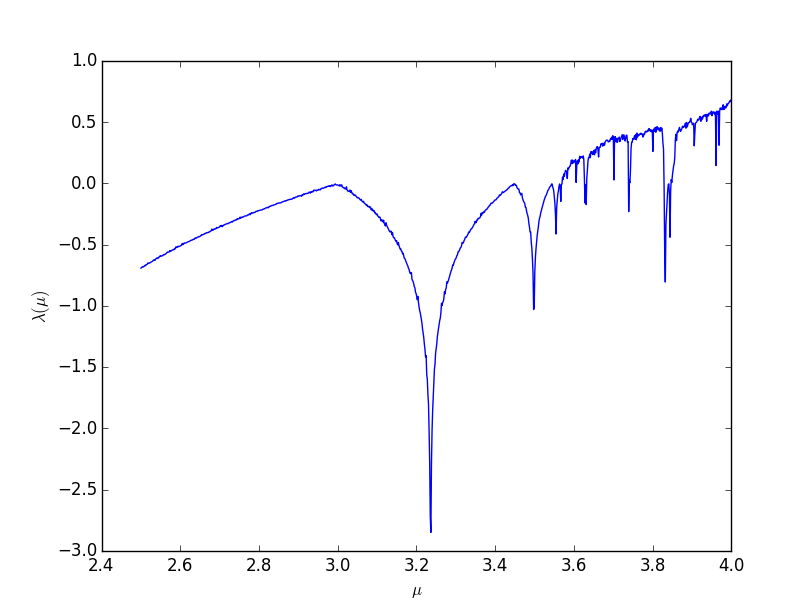
\includegraphics[width=0.88\textwidth]{Lyapunov-logistic.png}
\end{center}

\begin{itemize}
    \item Regiones con $\lambda<0$: predominan órbitas regulares.
    \item Cruces por $\lambda=0$: suelen marcar transiciones importantes.
    \item Regiones con $\lambda>0$: aparecen bandas caóticas.
\end{itemize}
\end{frame}

\begin{frame}[fragile]{Código base para calcular $\lambda(\mu)$}
\inputminted{python}{lyapunov.py}
\end{frame}

\begin{frame}[fragile]{Sugerencias de mejora para el código}
\begin{itemize}
    \item usar una semilla fija para reproducibilidad;
    \item descartar las primeras iteraciones antes de acumular la suma;
    \item evitar evaluar $\log(0)$ si $x_n=1/2$ en algún paso por redondeo;
    \item encapsular la simulación en funciones para reutilizarla luego.
\end{itemize}

\vspace{0.2cm}
\begin{block}{Pregunta para discutir}
¿Por qué dos sistemas que obedecen la misma ecuación, pero parten desde $x_0$ ligeramente distinto, pueden volverse impredecibles a largo plazo?
\end{block}
\end{frame}

\begin{frame}[fragile]{Actividad guiada: bifurcación y caos}
\small
\textbf{Parte práctica sugerida}
\begin{enumerate}
    \item correr el código del diagrama de bifurcación;
    \item identificar visualmente zonas periódicas y zonas caóticas;
    \item comparar el diagrama con el gráfico de $\lambda(\mu)$;
    \item elegir algunos valores de $\mu$ y describir la dinámica observada.
\end{enumerate}

\vspace{-0.5cm}
\inputminted{python}{logistic-bifurcation.py}
\end{frame}

\begin{frame}{Cierre de la Clase 1}
\begin{block}{Ideas que deben quedar claras}
\begin{itemize}
    \item El caos no significa azar puro: el sistema sigue siendo determinista.
    \item El exponente de Lyapunov cuantifica la sensibilidad a las condiciones iniciales.
    \item El mapa logístico es un laboratorio simple para estudiar transiciones complejas.
\end{itemize}
\end{block}

\textbf{Mini tarea sugerida:} estimar $\lambda(\mu)$ para una malla más fina de valores de $\mu$ y comparar con el diagrama de bifurcación.
\end{frame}

\section{Clase 2}

\begin{frame}{Clase 2: objetivos}
\textbf{Teoría breve}
\begin{itemize}
    \item introducir la entropía de Shannon como medida de dispersión/probabilidad;
    \item conectar histogramas con distribuciones discretizadas;
    \item formular el modelo de Lotka--Volterra y su resolución numérica con RK4.
\end{itemize}

\vspace{0.2cm}
\textbf{Programación}
\begin{itemize}
    \item construir histogramas y estimar entropía a partir de datos;
    \item implementar RK4 para un sistema de dos ecuaciones acopladas;
    \item visualizar trayectorias temporales y retratos de fase.
\end{itemize}
\end{frame}

\begin{frame}{Entropía de Shannon}
Para una distribución discreta $\{p_i\}_{i=1}^N$,
\begin{equation*}
    S = -\sum_{i=1}^{N} p_i \ln p_i,
    \qquad
    \sum_{i=1}^{N} p_i = 1.
\end{equation*}

\begin{itemize}
    \item Si la probabilidad está muy concentrada en pocos estados, $S$ es menor.
    \item Si la distribución es más uniforme, $S$ aumenta.
    \item El valor máximo ocurre cuando $p_i=1/N$ para todo $i$, y entonces $S_{\max}=\ln N$.
\end{itemize}
\end{frame}

\begin{frame}{Entropía estimada desde datos}
En una simulación, muchas veces no conocemos la distribución exacta. En su lugar:
\begin{enumerate}
    \item generamos una muestra de datos $x_1,\dots,x_M$;
    \item dividimos el intervalo de interés en $N$ bins;
    \item contamos cuántos datos caen en cada bin;
    \item normalizamos para obtener una aproximación $p_i$;
    \item calculamos $S = -\sum_i p_i \ln p_i$.
\end{enumerate}

\begin{block}{Idea práctica}
La elección del número de bins influye en el valor numérico de la entropía estimada. Esto permite discutir discretización, resolución y sesgo estadístico.
\end{block}
\end{frame}

\begin{frame}{Comparación visual de histogramas}
\begin{columns}[T,onlytextwidth]
\column{0.5\textwidth}
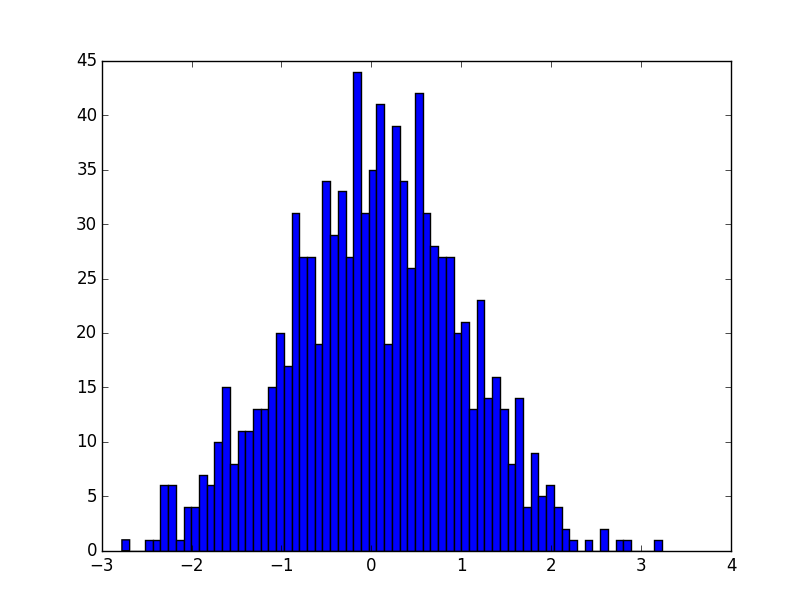
\includegraphics[width=\textwidth]{Entropy1.png}
\begin{center}
Distribución más extendida\\
$S\approx 2.63$
\end{center}
\column{0.5\textwidth}
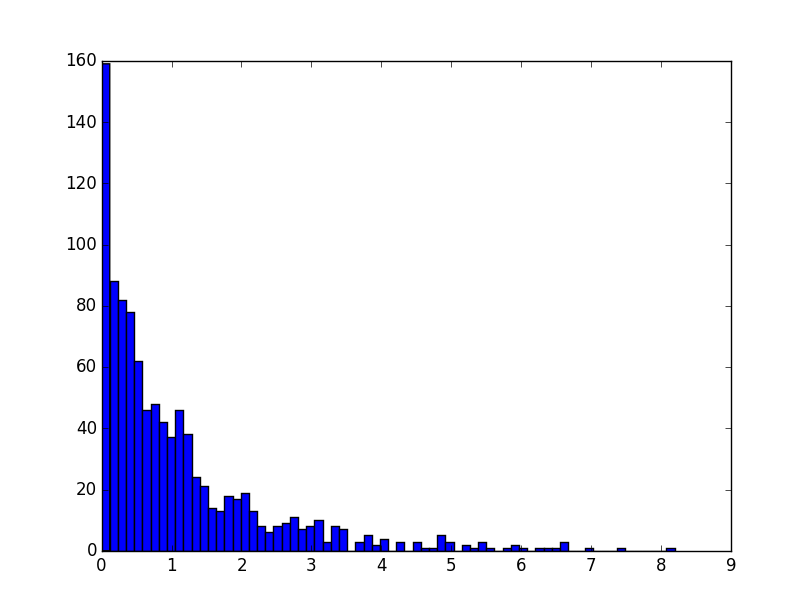
\includegraphics[width=\textwidth]{Entropy2.png}
\begin{center}
Distribución más concentrada\\
$S\approx 2.30$
\end{center}
\end{columns}
\end{frame}

\begin{frame}[fragile]{Función base para entropía}
\inputminted{python}{shannon.py}
\end{frame}

\begin{frame}{Modelo de Lotka--Volterra}
Sea $n_1(t)$ la población de presas y $n_2(t)$ la de depredadores. El modelo clásico es
\begin{align*}
    \frac{dn_1}{dt} &= a n_1 - b n_1 n_2, \\
    \frac{dn_2}{dt} &= c n_1 n_2 - m n_2.
\end{align*}

\begin{itemize}
    \item $a$: crecimiento natural de las presas;
    \item $b$: tasa de captura por interacción presa-depredador;
    \item $c$: eficiencia reproductiva del depredador;
    \item $m$: mortalidad natural del depredador.
\end{itemize}
\end{frame}

\begin{frame}{¿Por qué necesitamos integración numérica?}
El sistema de Lotka--Volterra es no lineal y acoplado. Aunque su estructura es simple, en un curso introductorio es más útil resolverlo numéricamente para:
\begin{itemize}
    \item estudiar trayectorias para distintos parámetros;
    \item comparar métodos numéricos;
    \item visualizar retratos de fase y oscilaciones.
\end{itemize}

Usaremos Runge--Kutta de orden 4 (RK4), uno de los métodos estándar para ecuaciones diferenciales ordinarias.
\end{frame}

\begin{frame}{Esquema RK4}
Para el problema
\begin{equation*}
    \dv{y}{t}=f(y,t), \qquad y(t_0)=y_0,
\end{equation*}
el paso de RK4 con tamaño $h$ es
\begin{align*}
    k_1 &= f(y_n,t_n), \\
    k_2 &= f\left(y_n+\frac{h}{2}k_1,t_n+\frac{h}{2}\right), \\
    k_3 &= f\left(y_n+\frac{h}{2}k_2,t_n+\frac{h}{2}\right), \\
    k_4 &= f\left(y_n+h k_3,t_n+h\right), \\
    y_{n+1} &= y_n + \frac{h}{6}(k_1+2k_2+2k_3+k_4).
\end{align*}

\begin{block}{Intuición}
RK4 promedia varias pendientes dentro del intervalo $[t_n,t_n+h]$ y logra muy buena precisión para pasos moderados.
\end{block}
\end{frame}

\begin{frame}[fragile,shrink=8]{Código base: Lotka--Volterra con RK4}
\inputminted{python}{lotka1.py}
\end{frame}

\begin{frame}{Resultados esperados}
\begin{columns}[T,onlytextwidth]
\column{0.52\textwidth}
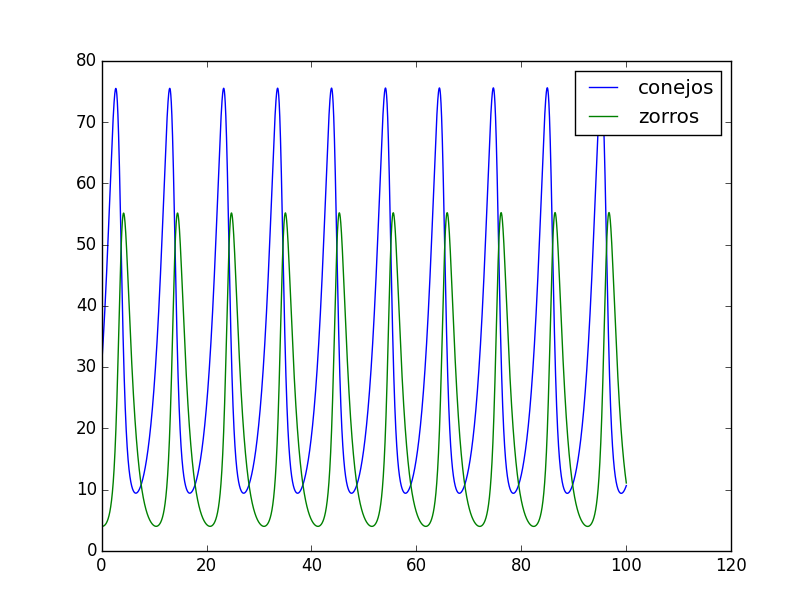
\includegraphics[width=\textwidth]{LV1.png}
\begin{center}
Evolución temporal de poblaciones
\end{center}
\column{0.44\textwidth}
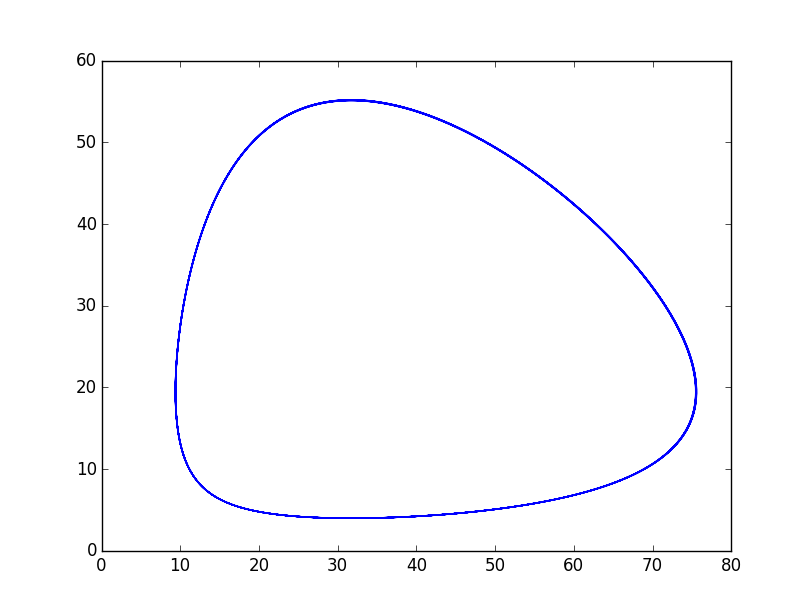
\includegraphics[width=\textwidth]{LV-phase.png}
\begin{center}
Retrato de fase $(n_1,n_2)$
\end{center}
\end{columns}
\end{frame}

\begin{frame}{Extensión a muchas especies}
Una generalización posible es
\begin{equation*}
    \frac{dn_i}{dt}=a_i n_i\left(1-\sum_{j=1}^{N} b_{ij}n_j\right), \qquad i=1,\dots,N.
\end{equation*}

Este tipo de sistemas permite explorar:
\begin{itemize}
    \item competencia entre especies;
    \item coexistencia y extinción;
    \item sensibilidad a parámetros e inestabilidades numéricas.
\end{itemize}

\begin{alertblock}{Desafío opcional}
Implementar RK4 para $N=4$ especies y estudiar proyecciones del espacio de fases, por ejemplo $(n_1,n_3)$ o $(n_2,n_4)$.
\end{alertblock}
\end{frame}

\begin{frame}{Actividades integradas de la semana}
\begin{enumerate}
    \item calcular el exponente de Lyapunov del mapa logístico para $\mu\in[2.5,4]$;
    \item construir o mejorar el diagrama de bifurcación del mapa logístico;
    \item estimar la entropía de Shannon de muestras generadas por una simulación;
    \item resolver el sistema Lotka--Volterra con RK4 y graficar $n_1(t)$, $n_2(t)$ y $n_1$ vs. $n_2$.
\end{enumerate}

\vspace{0.2cm}
\begin{block}{Criterio de avance}
Cada actividad debe incluir: código legible, parámetros claramente identificados, gráfico bien rotulado e interpretación física breve.
\end{block}
\end{frame}

\begin{frame}{Cierre de la semana}
\textbf{Conexión conceptual}
\begin{itemize}
    \item el mapa logístico muestra cómo reglas simples generan caos;
    \item la entropía de Shannon resume cuán dispersa está una distribución;
    \item Lotka--Volterra conecta modelamiento físico/matemático con integración numérica.
\end{itemize}

\vspace{0.3cm}
\begin{center}
\Large{Semana 02 = dinámica no lineal + medidas de complejidad + simulación}
\end{center}
\end{frame}

\end{document}
